\chapter{Characterization}
\graphicspath{{../gfx/chapter03/}{../plots/chapter03/}}


\section{The three-cell wire}

%
\begin{figure}
  \center
  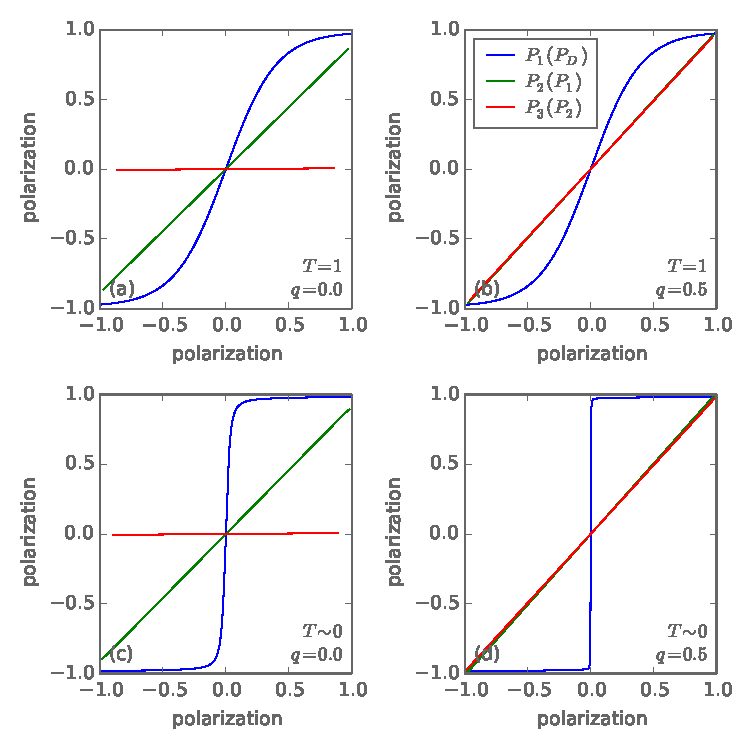
\includegraphics{three_cells_PP}
  \caption{
  The cell-cell polarization response. The response of the first cell with
  respect to the driver cell is non-linear and exhibits gain. In contrast, the
  response of the second cell with respect to the first cell, and similarly
  for the third with respect to the second, is linear and without gain. At zero
  temperature, the responses are generally improved, but the qualitative
  behaviour remains the same.
  }
  \label{fig:three_cells_PP}
\end{figure}
%
We choose a simple QCA system, the three-cell wire that we had already
introduced in Fig.~\ref{fig:short_wire}(b) in the first chapter, to investigate
general time-independent characteristics of QCA circuits. Specifically, we are
interested in how the polarization of one cell \emph{responds} to the
polarization of a second cell, and how cell polarizations depend on cell-cell
distance and inter-cell angle. For the three-cell wire we use a
nearest-neighbour Coulomb repulsion $V_1 = 40$ and the cell-cell distance is
$d/a = 2.2$, where $a$ is the edge length of the cell. Most of our calculations
will be at finite temperature, $T = 1$, and we will concentrate on horizontal
wires for now (meaning the inter-cell angle is $\theta = 0^{\circ}$). Both the
Coulomb energy scale $V_1$ and the temperature $T$ are in units of the hopping $t$,
with $t = 1$. For these parameters the bond approximation is valid, which we
deploy unless otherwise noted. We investigate systems both without compensation
charges $q = 0$, here the net cell charge is $-2e$, and with a compensation
charge of $q=\frac{1}{2}$, yielding charge-neutral cells.

The driver cell sets the input for the three-cell wire with its
polarization $P_D$ taking values in the range $-1$ to $+1$. The three active
cells respond to the driver polarization. For our discussion, we define the
linear polarization response of cell $k$ with respect to cell $l$ as
%
\begin{equation}
  \label{eq:polarization_response}
  \chi_{kl} = \frac{\partial P_k}{\partial P_l}\big|_{P_l = 0} \, .
\end{equation}
%
Fig.~\ref{fig:three_cells_PP}(a)~and~(b) show the polarization of the first cell
with respect to the driver cell, the polarization of the second cell with
respect to the first cell, and so on. For the first cell, the response is
non-linear and shows gain, therefore $\chi_{1D} > 1$. In contrast, the
polarization response between cells interior to the wire is linear and does not
exhibit gain, i.e.\ $\chi_{21} \le 1$ and $\chi_{32} \le 1$. Generally, the
polarization decreases monotonically from cell to cell, $|P_D| \ge |P_1| \ge
|P_2| \ge |P_3|$. In fact, for the $q=0$ system the polarization rapidly drops
to zero for the chosen parameters. The transmission is much improved for charge
neutral cells. In that case, the response is almost perfect, $\chi_{21} \sim
\chi_{32} \sim 1$.

It is worth pointing out that at zero temperature, where we have to use the
fixed charge model rather than the inapplicable bond approximation, we observe
the same polarization response characteristics, as demonstrated in
Fig.~\ref{fig:three_cells_PP}(c)~and~(d). Quantitatively, for the same system
parameters the response is improved at zero temperature compared to $T=1$. For
example, the first cell's polarization response becomes a near-perfect step
function for the chosen parameters. But, importantly, it remains true that the
response inside the wire ($\chi_{21}, \chi_{32}$) is always linear and without
gain. Without compensation charges, the polarization of the third cell remains
zero even in the ground state, indicating that the cells are so closely spaced
that charge buildup pushes the electrons of the rightmost cell to the rightmost
edge.

In the literature, the non-linear nature of $P_1(P_D)$ has been noted
\cite{lent1993quantum} \cite{lent1993lines}, and the apparent gain $\chi_{1D} >
1$ has been invoked to argue for the robustness and fault-tolerance of the QCA
scheme. However, as our graph shows, this is only strictly true for the response
with respect to the driver cell. We believe that the picture where each cell
switches with gain with respect to its neighbours is an artifact of the
intercellular Hartree approximation (ICHA), which we had introduced in more
detail in chapter \ref{ch:QCA_intro}. ICHA treats each cell individually in the
static charge mean field of the other cells in the system. In other words, in
the ICHA scheme, for each cell the rest of the system is approximated by an
effective driver cell.

%
\begin{figure}
  \center
  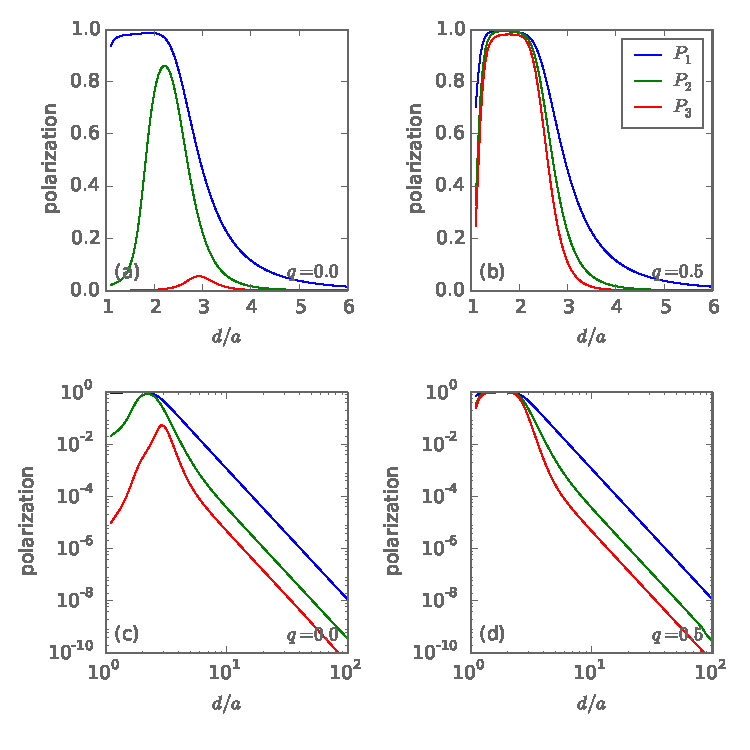
\includegraphics{three_cells_P_over_d}
  \caption{
  (a)(b)~Cell polarization over cell-cell distance. In the non-charge-neutral
  system ($q = 0$), due to charge buildup the maximum polarization for
  consecutive cells is at increasingly large cell-cell distances. Even at
  optimal distance the output polarization $P_3$ is very small. The output
  polarization is drastically improved for the charge-neutral system. Each cell
  attains its optimal polarization in the same range of cell-cell distances.
  (c)(d)~Cell polarization over very large cell-cell distances. For large
  distances $d/a > 10$ the polarizations settle into an universal long distance
  tail $d^{-5}$, independent of $q$ and as predicted by the Ising interaction
  $J$.
  }
  \label{fig:three_cells_P_over_d}
\end{figure}
%
We now fix the driver polarization at $P_D = 1$ and look at how the
polarizations of the active cells depend on the cell-cell distance $d/a$, see
Fig.~\ref{fig:three_cells_P_over_d}(a)~and~(b). At $d/a = 2$ all quantum dots in
the system are equally spaced, cells are placed a distance $a$ apart. At this
separation and smaller, our basic assumption of no inter-cell hopping breaks
down, as some dots in adjacent cells are now placed closer together than the
dots inside each cell. Thus $d/a \le 2$ is an unphysical limit. Conversely, at
very large cell-cell distances we expect the cells to become decoupled and
therefore all polarizations to be zero. Obviously, neither extreme limit is of
interest if our aim is to build functional QCA devices.

As already observed above, and in line with our intuition, polarizations
generally decrease from cell to cell as we go further away from the driver cell.
Without compensation charges ($q=0$) the polarization quickly falls off to very
small values, whereas for charge neutral cells ($q = \frac{1}{2}$) the situation
is much improved. The graph shows that there is a cell-cell distance that yields
maximal polarization for each cell. For the $q=0$ system---non-charge-neutral
cells---the optimal distance increases from cell to cell, due to charge buildup.
In contrast, with charge-neutral cells ($q=\frac{1}{2}$) the cell-cell distance
yielding optimal polarization does not change notably from cell to cell. In
fact, here a range of distances gives very good polarizations, as the
polarization saturates at values close to $P = 1$. Outside of this plateau
region cell polarizations still fall off quickly towards zero, for example for
cell-cell distances $d/a \gtrsim 3$. Of course, for a wire what really matters
is the output polarization. For the chosen parameters, this calculation
demonstrates that for a $q=0$ system we should choose $d/a \sim 2.9$. For
$q=\frac{1}{2}$ the range $d/a \sim 1.3 \ldots 2.3$ gives the best output
polarization. Worryingly, this range is very close to the lower, unphysical
limit!

Especially for the non-charge-neutral system it is beneficial to allow for
different distances between different adjacent cells along the wire. Thus a
single $d/a$ parameter is replaced by $d_k/a$ with $k = 1,2,3$ for the
three-cell wire. Using a stochastic optimization scheme introduced by Sandvik
\emph{et al}.\ \cite{Sandvik2007}, we can optimize the $d_k/a$ for optimal
output polarization. We find that the output polarization is significantly
improved from $P_3 = 0.06$ for uniformly spaced cells to $P_3 = 0.15$ for cells
with individual cell-cell distances. Not surprisingly, cells are farther spaced
to the right (the output) and closer spaced to the left (the input). This is a
manifestation of charge buildup in the system. The situation is very similar for
longer wires and different parameters for non-charge-neutral wires. Of course,
non-uniformely spaced cells have implications for the directionality of
transport in a wire, which would have to be considered when designing QCA
circuitry. More generally, we should be able to optimize the functionality of
any given non-charge-neutral QCA layout by allowing for slightly adjustable cell
placement. We can do the same stochastic optimization for charge-neutral wires
($q=1/2$), but find that little is gained by allowing non-uniform cell-cell
distances. Looking at Fig.~\ref{fig:three_cells_P_over_d} this is really not
surprising at all, and simply a consequence of having no charge buildup in the
system. It should be emphasized how much better the output polarization is for
charge-neutral wires. At least for the chosen parameters, even very short wires
seem unrealistic for a non-charge-neutral system.
% TODO: appendix with details on stochastic optimization?

It is instructive to plot the polarizations over cell-cell distance up to very
large distances in a log-log graph as shown in
Fig.~\ref{fig:three_cells_P_over_d}(c)~and~(d). Even though large distances come
with extremely small polarizations that are not of practical interest, this
graph yields valuable insights into the nature of the interaction that mediates
the polarization. At distances $d/a > 10$ we see that the polarization settles
into an universal long range tail with $P(d) \sim d^{-5}$. This is consistent
with our understanding that the polarization is mediated by a
quadrupole-quadrupole interaction. For these large distances the polarization is
exactly the same for both the $q=0$ and the $q=\frac{1}{2}$ systems. Hence,
having non-charge-neutral cells does not actually alter the characteristics of
the cell-cell interaction. Instead, it suppresses the cell-cell interaction at
small distances. That is, charge repulsion competes with the quadrupole
interaction. The graph exactly confirms our analysis from chapter
\ref{ch:approximations}. There, we had derived an approximate expression for the
mediating cell-cell interaction in the Ising picture, $J \sim d^{-5}$, to
leading order, and the derived $J$ was independent of $q$. At the time we had
seen that, in general, we can only map QCA to a modified Ising model with an
additional cell-cell interaction $J^{\prime}$, which does depend on $q$.
However, for the horizontal wire $J^{\prime}$ vanishes and we are left with the
pure Ising model, and at large enough distances the behaviour of the
polarization is just as predicted. Of course, we are mostly interested in small
distances, where the polarization is relatively large. Here, the polarization
falls off faster than $d^{-5}$ and, remembering the derivation of $J$, we would
need to include higher order corrections in the multipole expansion to
accurately describe this behaviour. Even with higher order terms the Ising model
and its $J$ cannot, however, correctly reproduce the suppression of the
quadrupole interaction at short distances in the case of $q=0$.

%
\begin{figure}
  \center
  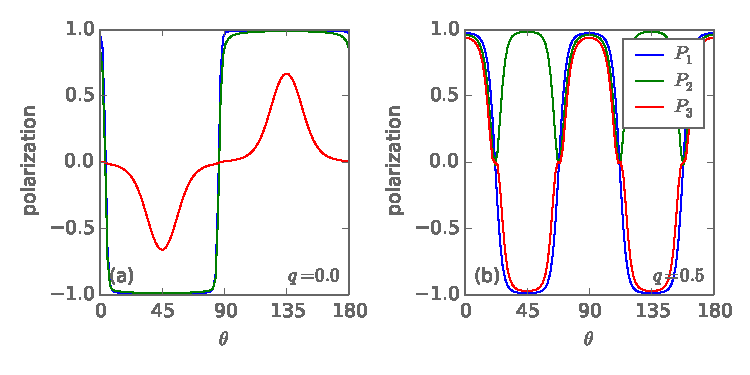
\includegraphics{three_cells_P_over_theta}
  \caption{
  Cell polarization over the inter-cell angle. The charge-neutral system is
  invariant under rotations by $90^{\circ}$ and closely matches the behaviour
  predicted by the Ising $J$. At $45^{\circ}$ cell polarizations are
  alternating. For the non-charge-neutral system, the polarizations are
  predominantly set by the angle, and not by the driver polarization. The system
  is invariant under rotations by $180^{\circ}$, as predicted by the modified
  Ising $J^{\prime}$. In the non-charge-neutral case QCA does not work at all,
  except for horizontal or vertical wires.
  }
  \label{fig:three_cells_P_over_theta}
\end{figure}
%
From the discussion of the Ising model in chapter \ref{ch:approximations}, we
already know that cell polarizations should change with the inter-cell angle.
The polarizations are mediated by the cell-cell interactions $J$ and
$J^{\prime}$, and specifically we had found $J \sim \cos{4 \theta}$, whereas
$J^{\prime} \sim \sin{2 \theta}$. We rotate the three-cell wire from a
horizontal configuration ($\theta = 0^{\circ}$) over diagonal ($\theta =
45^{\circ}$) to vertical ($\theta = 90^{\circ}$), and back to horizontal
($\theta = 180^{\circ}$), and look at the cell polarizations in the process.
Fig.~\ref{fig:three_cells_P_over_theta}(b) shows the polarization as a function
of the angle for the charge-neutral system, where $J^{\prime} = 0$. Indeed, the
cell polarizations follow the behaviour predicted by $J$: they are rotationally
invariant under rotations by $90^{\circ}$ and peak at the angles $0^{\circ},
90^{\circ}$, and so on, where $J > 0$. At $45^{\circ}$, where $J < 0$, cell
polarizations are alternating, e.g.~$P_D \sim 1$, $P_1 \sim -1, P_2 \sim 1$, and
$P_3 \sim -1$. In between, for example at $\theta = 22.5^{\circ}$, $J = 0$ and
the polarization is zero accordingly. The wire can be used to transmit signals
in a range of about $20^{\circ}$ around $\theta = n \cdot 45^{\circ}$, where $n$
is an integer and the usable angle range depends on the chosen system
parameters. Of course, at $45^{\circ}$ we have to make sure to use an even
number of cells for transmission, as the signal will be inverted otherwise.
Conceivably, the nodes at $22.5^{\circ}, 67.5^{\circ}$, and so on could be used
to decouple closely spaced cells.

The situation is very different for non-charge-neutral systems, as shown in
Fig.~\ref{fig:three_cells_P_over_theta}(a). In this case, $J^{\prime} \ne 0$ and
we see that the polarization is actually predominantly set by $J^{\prime}$,
which is rotationally invariant under rotations by $180^{\circ}$. This is in
line with our derivation where we had found, to leading order, $J^{\prime} \sim
d^{-3}$, whereas $J \sim d^{-5}$, and thus, $J^{\prime}$ was expected to
dominate. The graph shows that the cell polarizations are much larger in
magnitude away from $0^{\circ}, 90^{\circ}$, and so on, where we know that the
system behaves as expected. In fact, the presented graph looks exactly the same
for $P_D = 1$ and $P_D = -1$, except for a small range of angles of about
$5^{\circ}$ around $\theta = n \cdot 90^{\circ}$, where the angle range again
depends on the chosen system parameters. In short, the cells' polarizations are
set by the inter-cell angle, and not by the driver polarization. The importance
of charge neutrality had first emerged in our discussion of the Ising model.
Here we see this finding most impressively confirmed. The non-charge-neutral
system will never work as a QCA circuit unless all we want to do is build linear
chains of cells. Even in this case the system becomes very fragile with respect
to angular displacement. Thus, for QCA charge-neutral cells, $q=\frac{1}{2}$,
are absolutely essential. In the literature charge neutrality has usually been
assumed, either explicitly or implicitly, but as far as we know, no one else has
previously identified its crucial role.


\section{Workable parameters for QCA}

\begin{figure}
  \center
  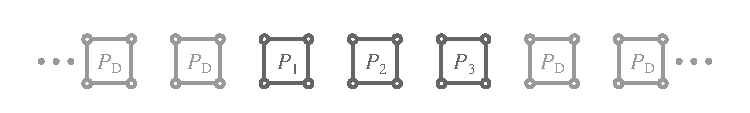
\includegraphics{semi_infinite_wire}
  \caption{
  }
  \label{fig:semi_infinite_wire}
\end{figure}

\begin{figure}
  \center
  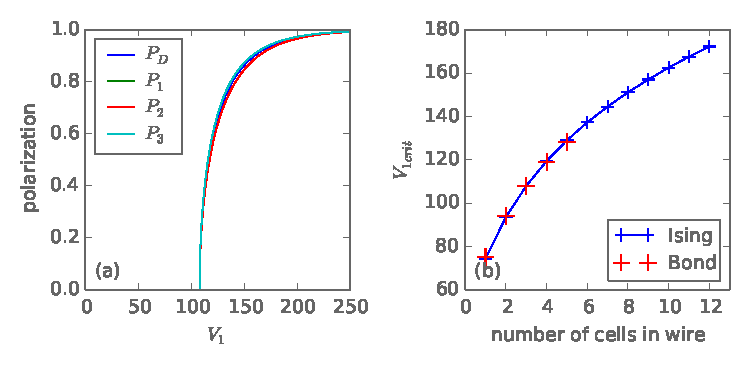
\includegraphics{critical_V1}
  \caption{
  }
  \label{fig:critical_V1}
  % TODO: change caption of (b): is should be "number of active cells"
\end{figure}

\begin{table}
  \center
  \begin{tabular}{c c r @{.} l p{0cm} c c r @{.} l}
    $T$ & $d/a$ & \multicolumn{2}{c}{$V_{1crit}$} & &
    $T$ & $d/a$ & \multicolumn{2}{c}{$V_{1crit}$} \\
    \hline 
    $1$ & $2.2$ & $ 14$&$71$ & &
    $2$ & $2.2$ & $ 25$&$99$ \\
    $1$ & $3.0$ & $ 55$&$10$ & &
    $2$ & $3.0$ & $107$&$90$ \\
    $1$ & $4.0$ & $230$&$24$ & &
    $2$ & $4.0$ & $459$&$87$ \\
  \end{tabular}
%  \begin{tabular}{c c r @{.} l}
%    $T$ & $d/a$ & \multicolumn{2}{c}{$V_{1crit}$} \\
%    \hline 
%    $1$ & $2.2$ & $ 14$&$71$ \\
%    $1$ & $3.0$ & $ 55$&$10$ \\
%    $1$ & $4.0$ & $230$&$24$ \\
%    $2$ & $2.2$ & $ 25$&$99$ \\
%    $2$ & $3.0$ & $107$&$90$ \\
%    $2$ & $4.0$ & $459$&$87$ \\
%  \end{tabular}
  \caption{
  }
  \label{tab:critical_V1}
\end{table}

In the previous section we found charge-neutral cells to be essential for QCA.
Therefore we will from now on restrict ourselves to $q=\frac{1}{2}$ systems.
Additionally, we saw that in a line of cells the polarization is at best
preserved but generally decreases from cell to cell. There is no inter-cell
gain. If the cell-cell polarization response is less than ideal then the
polarization will eventually decrease to zero for a long line of cells,
rendering the wire non-functional. It is therefore important to identify a
parameter regime where the response is ideal or close-to-ideal as a prerequisite
for functional QCA circuits.

% TODO: more motivation why I want to calculate semi-infinite wires in the first
% place?
We use a cluster mean field approach beyond the single-site ICHA approximation
to calculate the polarizations of semi-infinite wires. A small cluster of active
cells is embedded in a large number of driver cells---the mean field---whose
polarization is set as the average of the active cells. The setup is illustrated
in Fig.~\ref{fig:semi_infinite_wire}, for three active cells. Therefore, instead
of solving only the one-cell mean field Hamiltonian $H^{\mathrm{MF}}_k$
\eqref{eq:H_meanfield} introduced in section \ref{sec:basic_characterization},
as for the ICHA scheme, we solve a cluster mean field Hamiltonian
$H^{\mathrm{MF}}$, and instead of only using a single cell's polarization $P_k$,
the average of all active cells $\left< P_k \right>$, obtained from
$H^{\mathrm{MF}}$, is used to set the mean field $P_D$. The self-consistency
condition then is
%
\begin{equation}
  P_D = \left< P_k \left( P_D \right) \right> \, .
\end{equation}
%
If we don't find a solution for the self-consistency condition for a given set
of parameters then only the trivial solution $P_D = 0$ remains. In this case no
self-consistent polarization exists.

We made a point of how problematic mean field approximations can be. Here we use
the approach to establish a \emph{lower bound} on workable parameters. In
principle, the number of active cells can be indefinitely increased and
properties of interest can be extrapolated to the thermodynamic limit; the
approximation is asymptotically correct. Of course, in practice the number of
active cells allowed by the available computer resources is actually quite small
and probably far from the asymptotic behaviour. We have found that as few as ten
driver cells on each side of the active cells already look like an infinite
wire. Adding more and more driver cells the active cells' polarizations quickly
saturates, indicating that they don't ``see'' cells farther away than ten cells.
This also shows that in practice the interaction, while beyond
nearest-neighbour, is not extremely long-ranged. In the following calculations
we use 100 driver cells on each side of the active cells.

We go back to the horizontal three-cell wire, but now use a larger cell-cell
distance $d/a = 3.0$ and a higher temperature $T = 2$, and calculate the
self-consistent polarization over a wide range of values of $V_1$, shown in
Fig.~\ref{fig:critical_V1}(a). We observe a second-order phase transition at
$V_{1crit}$. For $V_1 < V_{1crit}$ no self-consistent solution with $P_D > 0 $
exists. This regime is therefore inhibitive for QCA devices. Above the critical
$V_1$ the polarization rises very sharply and quickly saturates towards full
polarization. The presence of a phase transition is likely an artifact of the
mean field method. Still, the scale of the critical $V_1$ sheds light on what
order of magnitude to expect for a workable $V_1$. For our system, we find that
$V_1 \gtrsim 150$ should yield large cell polarizations, and as before this is
in units of the hopping, with $t = 1$. For more favourably chosen parameters the
critical $V_1$ can also be much smaller. Table~\ref{tab:critical_V1} lists the
$V_{1crit}$ for a variety of different system parameters. In particular, for the
parameters used for the three-cell wire in the last section, $T = 1$ and $d/a =
2.2$, the critical $V_1$ is only $V_{1crit} = 14.71$. The table also
demonstrates that the critical $V_1$ grows very rapidly for larger cell-cell
distances. This is in line with what we had seen in
Fig.~\ref{fig:three_cells_P_over_d}(a)~and~(b), where we had plotted the cell
polarizations as a function of the cell-cell distance. In that graph, after a
plateau-like feature at small distances, the polarization had dropped off very
quickly for growing inter-cell spacing. Both observations emphasize that small
cell-cell distances are crucial, and, generally, we want distances as small as
possible while still satisfying our underlying physical assumptions, such as no
inter-cell hopping. Let us note that a graph qualitatively similar in appearance
to Fig.~\ref{fig:critical_V1}(a), obtained from ICHA calculations for a
seven-cell wire, has been reported in the literature previously
\cite{Lent1993Lines}. However, the reference's interpretation of the graph is
lacking. In particular, the significance and consequences of employing a mean
field scheme was not understood, and the found critical values were therefore
not identified as lower boundaries, but taken at face value.

Without doubt the most pressing question is how the critical $V_1$ changes with
the number of active cells. Does $V_{1crit}$ exhibit a clear scaling behaviour?
Can we extrapolate to the thermodynamic limit? Fig.~\ref{fig:critical_V1}(b)
traces $V_{1crit}$ as the number of active cells is increased. With the more
accurate bond model only up to five cells are computationally feasible, and we
have therefore included calculations with the Ising model for up to twelve
active cells. For the chosen system parameters, the obtained values of the
critical $V_1$ are relatively large and the Ising model is therefore expected to
give sufficiently accurate results. Comparing the bond and Ising model in the
graph, we see that they indeed agree well. The bond model gives slightly larger
$V_{1crit}$ than the Ising model for one and two active cells, but for four and
five active cells the situation is reversed.  Therefore, extrapolating the
trend, we believe that the Ising model slightly overstimates the critical $V_1$
for at a larger number of active cells. This is in line with our observation in
section \ref{sec:validity_of_the_approximations} that the Ising model generally
underestimates the polarization. Most importantly, the graph shows that the
critical $V_1$ grows monotonically, and significantly, with an increasing number
of active cells. For the chosen parameters, the $V_{1crit}$ for twelve active
cells is more than twice the $V_{1crit}$ for only one active cells. The critical
$V_1$ grows more slowly for larger numbers of active cells, but does not
saturate, and there is no clear identifyable scaling behaviour otherwise.
Therefore, we are inclined to conclude that the $V_1$ grows indefinitely and
becomes infinite in the thermodynamic limit.
% TODO: Probably better to avoid explicit questions.
% TODO: more on what an infinite V_{1crit} means

\begin{figure}
  \center
  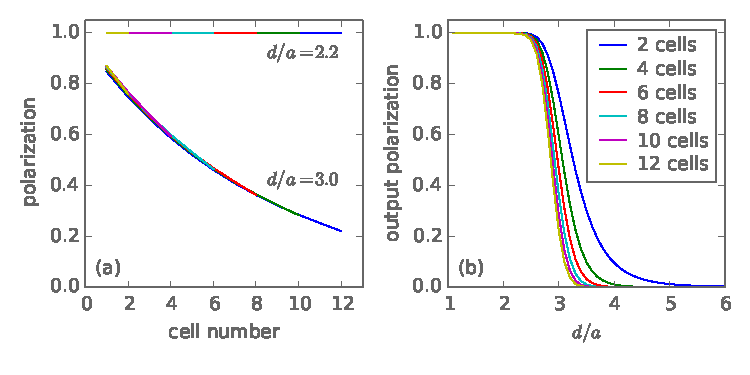
\includegraphics{wire_polarization}
  \caption{
  }
  \label{fig:wire_polarization}
\end{figure}

To put the found mean field $V_{1crit}$ values into perspective we calculate the
cell polarizations in two- to twelve-cell wires at $V_1 = 200$---well above all
the $V_{1crit}$ values in Fig.~\ref{fig:critical_V1}(b)---and with a driver
polarization of $P_D = 1$. According to Fig.~\ref{fig:critical_V1}(a), which was
calculated for three active cells, at $V_1 = 200$ we should have a
self-consistent average polarization of $\left< P_k \right> = 0.97$ throughout
the semi-infinite wire. However, in an actual wire the cell polarizations are
not constant, but drop off quickly and are also much smaller, as shown in
Fig.~\ref{fig:wire_polarization}(a) in the $d/a = 3.0$ curve. For a six-cell
wire the output polarization is already less than half of the input
polarization, for twelve cells it is almost a fifth. The graph strongly
suggests that the polarization will continue to drop to zero for longer wires.
It therefore becomes apparent that the mean field $V_{1crit}$ really does set a
lower boundary, and in practice significantly larger $V_1$ values are necessary
for functional QCA devices, even for relatively small systems.

Fig.~\ref{fig:wire_polarization}(a) also includes cell polarizations for wires
with a cell-cell distance $d/a = 2.2$. For these systems,
Table~\ref{tab:critical_V1} lists $V_{1crit} = 25.99$, which was determined for
three active cells in a semi-infinite wire and is presumably considerably larger
for a larger number of active cells. At $V_1 = 200$, we are therefore almost an
order of magnitude higher than the critical $V_1$. At these shorter cell-cell
distances the cell polarizations are essentially perfect for all two- to
twelve-cell wires. When we zoom in, however, we find that the behaviour is
qualitatively the same as for the $d/a = 3.0$ wires, the polarizations still
decrease monotonically along the wire. But quantitatively the short cell-cell
distances are quite a different story. The polarizations fall off so slowly,
that we can reasonably expect to achieve sufficiently large output polarizations
for very long wires.

The cell polarization curves for all two- to twelve-cell wires in
Fig.~\ref{wire_polarization}(a) almost lie on top of each other, implying that
the polarizations of existing cells are hardly change as the wire is made
longer by adding more cells to the right. We can inspect the cell polarization
responses along the wire $\chi_{i,i-1}$ and find that they are indeed almost
constant, with the exception of the first cell which responds to the driver cell and
therefore behaves slightly different, and the last two cells, which have
slightly lower responses, due to edge effects. We know that the cell
polarization responses interior to the wire are linear. Therefore, we are
inspired to fit the cell polarization curves to a simple physical model, 
%
\begin{equation}
  P_k = \chi_e \chi^k \, .
\end{equation}
%
Here, $P_k$ is the polarization of cell $k$ in the wire, $\chi$ is the
polarization response which is assumed to be the same for all cells in the wire,
and $\chi_e$ is the system response to the driver cell. If the response to the
driver cell was the same as for a regular cell, then we would have $\chi_e = 1$.
We fit this model to the polarization curves and find that it works surprisingly
well, as can be seen in Fig.~\ref{fig:wire_polarization}(b), where we have
plotted the fitted $\chi_e$ and $\chi$ for three- to twelve-cell wires. The
errors are on the order of $10^{-3}$ for $d/a = 3.0$ and $10^{-7}$ for $d/a =
2.2$. Generally, we find that $\chi_e$ decreases for longer and longer wires,
whereas $\chi$ increases every so slightly. If the model worked perfectly then
both parameters would be the same for all wires, which is arguably true for
$\chi$ and, to a lesser extend, also for $\chi_e$. Thus, given that the model is
so simple, we feel that it works reasonably well, and over a range of system
parameters. The assumption of constant cell responses throughout the wire starts
to break down for larger cell-cell distances $d/a \gtrsim 4$, where, however,
the actual polarizations are already very small for a majority of cells.
% by manual inspection we find: It is indeed the response to the driver cell
% that gets weaker for longer wires, the rest of the wire's response is still
% more or less constant


% TODO: maybe I should somehow discuss how meaningful the calculation of the
% V_{1crit} really is --- evidently, wire polarizations are not constant and the
% calculation of V_{1crit} kind of assumes that (assumes it implicitly); both
% plots---V_1crit going to infinity for larger systems and the polarization
% falling off so quickly in real, short wires---point to an interpretation that
% the polarization is not constant in real systems; it always falls off; this is
% in line with our simple model where we have P \sim \chi^i

% TODO: I probably also want an estimate, using my simple model and fit
% parameters, how large I can make a system with V_1 = 200 and d/a = 2.2 ---
% where the polarizations are very large indeed.

% TODO: I could include a P_out over d/a plot for 2- to 12-cell wires and the
% d/a over N plot where P > 0.8, for different V1 values; I could explain the
% wire polarization plot for d/a = 3.0,2.2, give estimates for what numbers of
% cells that can realistically be expected and then ask: Why is there such a big
% difference between d/a = 3.0 and d/a = 2.2; this would be answered with these
% plots.
% Should I mention that the exploration of the parameter space is in some ways
% limited by the Ising approximation (smaller V1 is not feasible)?


% TODO: This chapter should also include a section where we put put our
% abstract, unit-less results into context, by again discussing the silicon
% system as an example
